\documentclass[a4paper]{ltjsarticle}

\usepackage[dvipdfmx]{graphicx}
\usepackage[dvipdfmx,hidelinks,pdfusetitle]{hyperref}
\hypersetup{
    colorlinks=false,
    bookmarksnumbered=true,
    pdfborder={0 0 0},
    bookmarkstype=toc
}
\usepackage[nobreak]{cite}
\usepackage{pxjahyper}
\usepackage{amsmath}
\usepackage{tikz}

\usetikzlibrary{datavisualization}
\usetikzlibrary{positioning}
\usetikzlibrary{shapes.geometric, shapes.misc}
\usetikzlibrary{patterns}
\usetikzlibrary{calc}

\begin{document}

\begin{itembox}[l]{京都大学 2018年 文系 第1問}
    $a$ は正の実数とし,座標平面内の点 $(x_0, y_0)$ は2つの曲線

    \begin{equation*}
        C_1\colon y=|x^2-1|,\ C_2\colon y=x^2-2ax+2
    \end{equation*}

    の共有点であり, $|x_0|\neq 1$ を満たすとする. $C_1$ と $C_2$ が $(x_0,\ y_0)$ で共通の接点をもつとき, $C_1$ と $C_2$ で囲まれる部分の面積を求めよ.
\end{itembox}

$|x_0|>1$ とすると,

\begin{align*}
     & C_1\colon y=x^2-1\quad\text{より}\quad y'=2x        \\
     & C_2\colon y=x^2-2ax+2\quad\text{より}\quad y'=2x-2a
\end{align*}

よって,$2x_0=2x_0-2a$ が必要だが,これは $a>0$ に反する.ゆえに,$|x_0|<1$ である.したがって,

\begin{equation*}
    C_1\colon y=-x^2+1\quad\text{より}\quad y'=-2x
\end{equation*}

であり,$C_1$ と $C_2$ が $(x_0,\ y_0)$ で共通の接点をもつためには,

\begin{equation*}
    \begin{cases}
        -{x_0}^2+1={x_0}^2-2ax_0+2 \\
        -2x_0=2x_0-2a
    \end{cases}
\end{equation*}

$a>0$ より,

\begin{equation*}
    a=\sqrt{2},\ x_0=\frac{\sqrt{2}}{2}
\end{equation*}

このとき,

\begin{equation*}
    C_2\colon y=(x-\sqrt{2})^2
\end{equation*}

また,

\begin{equation*}
    x^2-1=x^2-2\sqrt{2}x+2\quad\Longleftrightarrow\quad x=\frac{3\sqrt{2}}{4}
\end{equation*}

以上より, $C_1$ と $C_2$ で囲まれる部分は下図の斜線部であり,その面積を $S$ とすると,

\begin{figure}[!ht]
    \centering
    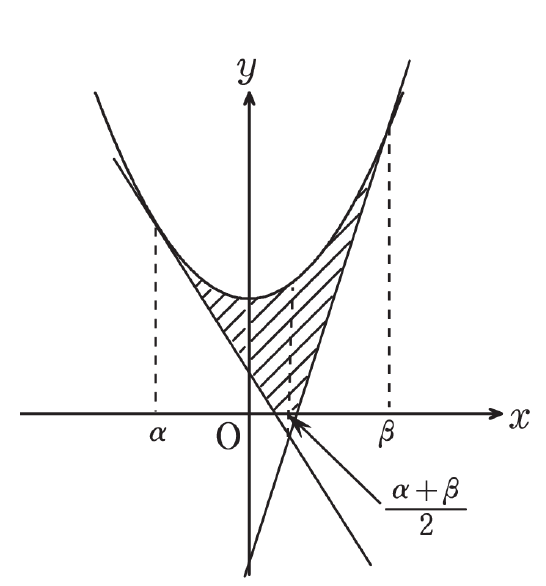
\includegraphics[width=100mm]{f1.png}
\end{figure}

\begin{align*}
    S & =\int_{\frac{\sqrt{2}}{2}}^1\left\{(x^2-2\sqrt{2}x+2)-(-x^2+1)\right\}dx+\int_1^{\frac{3\sqrt{2}}{4}}\left\{(x^2-2\sqrt{2}x+2)-(x^2-1)\right\} \\
      & =\left[\frac{2}{3}x^3-\sqrt{2}x^2+x\right]_{\frac{\sqrt{2}}{2}}^1+\left[\sqrt{2}x^2+3x\right]_1^{\frac{3\sqrt{2}}{4}}                          \\
      & =\left(\frac{5}{3}-\frac{7\sqrt{2}}{6}\right)+\left(\frac{17\sqrt{2}}{8}-3\right)                                                              \\
      & =\frac{23\sqrt{2}}{24}-\frac{4}{3}
\end{align*}

\end{document}
